\section{Definition}
Given:
\begin{itemize}
    \item $\mathcal{l}$, the length of the block;
    \item $\Sigma$, the alphabet;
\end{itemize}
A block cipher is a cryptosystem such that:
\[M = \mathcal{C} = \Sigma^{\mathcal{l}}\]
\begin{proposition}
    Consider waht follows:\newline
    The enciphering function of a block cypher is a permutation of $\Sigma^{\mathcal{l}}$.
\end{proposition}
\begin{proof}
    The proof proceeds as follows:
    \begin{itemize}
        \item Let $\mathcal{f}: \Sigma^{\mathcal{l}} \rightarrow \Sigma^{\mathcal{l}}$.
        \item Let $\mathcal{f}(m) = \mathcal{f}([p_{1}, p_{2}, \dots, p_{e}]) = \Pi(p_{1}, p_{2}, \dots, p_{e})$, where $p_{i} \in \Sigma$.
        \item Then, let $\mathcal{f}^{-1}(c) = \mathcal{f}([c_{1}, c_{2}, \dots, c_{e}]) = \Pi(c_{1}, c_{2}, \dots, c_{e})$, where $c_{i} \in \Sigma$.
        \item Let then $K_{E} = \Pi$ be the set of encyphering keys;
        \item Let then $K_{D} = \Pi^{-1}$ be the set of decyphering keys;
        \item Then, $|K| = (|\Sigma|^{\mathcal{l}})!$
        \item Due to the Pigeonhole principle, if $\mathcal{f}$ is injective, then it's also surjective, and therefore a bijection.
    \end{itemize}
\end{proof}

\section{Enciphering methods}
Since block cyphers encrypt just message of length $\mathcal{l}$, it's necessary to define the different ways in which the blocks can be used in order to compute the ciphertext.
\subsection{Electronic Code Book mode (ECB)}
Consider what follows:
\begin{itemize}
    \item Let $M \in \Sigma^{t}$ be the message, and $t = |M|$.
    \item Let $\mathcal{l}$ be the length of the block, such that $\mathcal{l} \nmid t \land t > \mathcal{l}$.
    \item $M$ is splited in blocks of length $\mathcal{l}$, and the remaining part is filled with garbage. This concatenation is called $M'$.
    \item $M'$ is sent to the receiver.
    \item If $M'$ is received in the correct order, the  message is received correctly.
\end{itemize}

\begin{figure}[h]
    \centering
    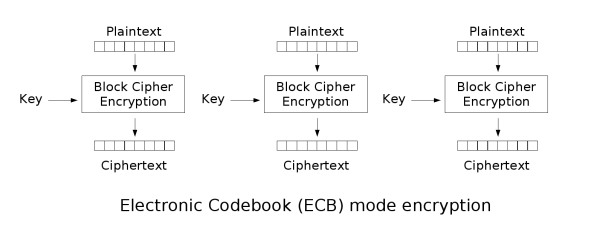
\includegraphics[width=0.75\textwidth]{img/ECB.png}
\end{figure}

\subsection{Cipher Block Chaining mode (CBC)}
This method introduces a XOR encryption to the communication. \newline
Consider what follows:
\begin{itemize}
    \item Let $\Sigma = \{0,1\}, M, C \in \{0,1\}^{\mathcal{l}}$
    \item Let $\oplus$ be the XOR operator (as known as the sum in $\mathbb{Z}_{2}$).
    \item Let $P \in \{0,1\}^{\mathcal{l}}$ the initial fixed plaintext, pre-agreed.
    \item Assume that $|M| = k \cdot \mathcal{l}$.
    \item Alice sends the ciphered message $C = [c_{0}, c_{1}, \dots, c_{k}]$ to Bob. That is:
    \begin{align*}
        \begin{cases}
          c_{0} & = \mathcal{f}(P)\\
          c_{j} & = \mathcal{f}(c_{j-1} \oplus m_{j}) \text{, for } 1 \leq j \leq k
        \end{cases}
    \end{align*}
    \item In order to receive correctly the message, it's important that Bob receives correctly $c_{0}$ and computes $\mathcal{f}^{-1}(c_{0})$. If that matches the original $P$, then he can proceed by computing the other blocks:
    \[m_{j} = c_{j-1} \oplus \mathcal{f}^{-1}(c_{j}), 1 \leq j \leq k\]
    This works because:
    \begin{align*}
        c_{1} = \mathcal{f}(c_{0} \oplus m_{i}) & \land c_{0} = \mathcal{f}(c_{0}) \\
        c_{0} \oplus \mathcal{f}^{-1}(c_{1}) & = c_{0} \oplus \mathcal{f}^{-1}(\mathcal{f}(c_{0 \oplus m_{1}})) \\
        & = c_{0} \oplus c_{0} \oplus m_{1} = m_{1}
    \end{align*}
\end{itemize}

\begin{figure}[h]
    \centering
    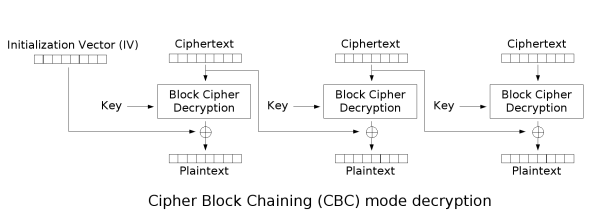
\includegraphics[width=0.75\textwidth]{img/CBC.png}
\end{figure}


\subsection{Cipher Feedback mode (CFB)}
Let the common knowledge of the communication be:
\begin{itemize}
    \item $P$ an initial value;
    \item $\mathcal{l}$, the length of the block.
    \item $1 \leq r \leq \mathcal{l}$ be a number.
\end{itemize}
Then, let $M = [m_{1}, \dots, m_{t}]$ be the cleartext message, where:
\[|m_{i}| = r \implies r | |M| \]
The communication is executed as follows:
\RestyleAlgo{ruled}
\begin{algorithm}
\caption{Cipher FeedBack Mode communication (CFB) [Sender]}\label{alg:CFB_sender}
$I_{1} \gets P \in \{0,1\}^{\mathcal{l}}$\;
\For{$j \in 1, \dots, t$}{
    $O_{j} \gets \mathcal{f}(I_{j})$\;
    $u_{j} \gets O_{j} \bmod 2^{r}$\;
    $c_{j} \gets m_{j} \oplus u_{j}$\;
    $I_{j+1} \gets 2^{r} I_{j} + c_{j} \bmod 2^{\mathcal{l}}$\;
}
\Return{$C$}
\end{algorithm}

\begin{figure}[h]
    \centering
    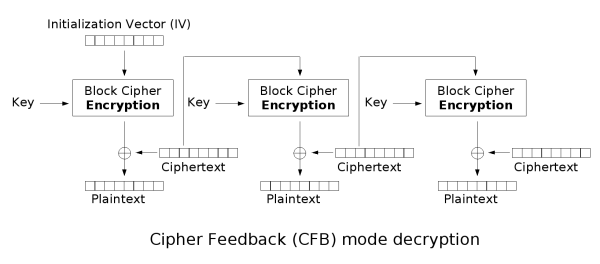
\includegraphics[width=0.75\textwidth]{img/CFB.png}
\end{figure}

\RestyleAlgo{ruled}
\begin{algorithm}
\caption{Cipher FeedBack Mode communication (CFB) [Receiver]}\label{alg:CFB_receiver}
$I_{1} \gets P $\;
\For{$j \in 1, \dots, t$}{
    $O_{j} \gets \mathcal{f}(I_{j})$\;
    $u_{j} \gets O_{j} \bmod 2^{r}$\;
    $m_{j} \gets c_{j} \oplus u_{j}$\;
    $I_{j+1} \gets 2^{r} I_{j} + c_{j} \bmod 2^{\mathcal{l}}$\;
}
\Return{$C$}
\end{algorithm}


\subsection{Output Feedback mode (OFB)}
Each output feedback block cipher operation depends on all previous ones, and so cannot be performed in parallel. However, because the plaintext or ciphertext is only used for the final XOR, the block cipher operations may be performed in advance, allowing the final step to be performed in parallel once the plaintext or ciphertext is available.
\begin{figure}[h]
    \centering
    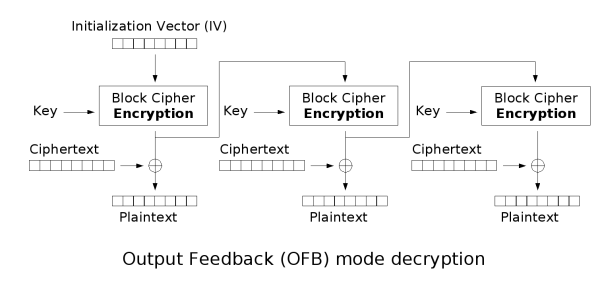
\includegraphics[width=0.75\textwidth]{img/OFB.png}
\end{figure}

\section{Feistel's Ciphers}
The Feistel's cipher cryptosystem is the predecessor of the DES. It is defined as follows:
\begin{align*}
    \Sigma = \{0,1\} \\
    \mathcal{M} = \mathcal{C} = \mathcal{K} = \Sigma^{\mathcal{l}}\\
    \mathcal{f}_{k}: \Sigma^{\mathcal{l}} \rightarrow \Sigma^{\mathcal{l}}\\
    \mathcal{F}_{k}: \Sigma^{2\mathcal{l}} \rightarrow \Sigma^{2\mathcal{l}}
\end{align*}
This cipher loops the enciphering function $F$ $r$ times, in which the blocks have a lenght of $2 \cdot \mathcal{l}$. $f$ is a sort of internal enciphering function. \newline
There's also a key generating function, that has the following signature:
\[\mathcal{K} \rightarrow \mathcal{K}^{r}\]
The algorithm enciphers as follows:
\begin{enumerate}
    \item The cleartext message $M$ is composed of two parts: $L_{0}, R_{0}$, where $|L_{0}| = |R_{0}| = \mathcal{l}$.
    \item Consider that $K_{i}$ is the $i$-th key produced.
    \item For every $i: 1 \leq i \leq r$, $C_{i}$ is computed:
    \[C_{i} = [L_{i}, R_{i}] = [R_{i-1}, L_{i-1} \oplus f_{K_{i}}(R_{i-1})\]
    \item The message that is sent is $F_{K_{r}} = [R_{r}, L_{r}]$
\end{enumerate}
The deciphering method proceeds as follows:
\begin{enumerate}
    \item Note that the keys must be used in reverse order.
    \item At each step, it is computed:
    \[R_{i} \gets L_{i-1} \oplus f_{K_{i}}(R_{i-1}), L_{i} \gets R_{i-1}\]
    \item Also, note that $f_{K_{i}} = f^{-1}_{K_{i}}$, since it's used with the XOR operator.
\end{enumerate}
An important remark is that the complexity of this algorithm depends on $f_{K}$

\section{Data Encryption Standard (DES)}
\subsection{Single DES}
The DES cryptosystem works as a Feistel's Cipher, where:
\begin{itemize}
    \item $\mathcal{l} = 32$ bits;
    \item $r = 16$ rounds;
\end{itemize}
Let now:
\begin{itemize}
    \item $\pi(b_{1}, \dots, b_{64}) = (b_{58}, b_{50}, b_{42}, \dots, b_{23}, b_{15}, b_{7})$ be a permutation;
    \item $E$ be an expansion;
    \item $S$ be a substitution;
    \item $P$ be a round permutation.
    \item Also, the set of the keys is defined as follows:
    \[\mathcal{K} = \{(b_{0}, b_{1}, \dots, b_{64}) \in \{0,1\}^{64}: \forall j \in \{0, 1, \dots,7\}: \sum_{i=1}^{8} b_{8j + i} \equiv_{2} 1\}\]
\end{itemize}

\RestyleAlgo{ruled}
\begin{algorithm}
\caption{Data Encryption Standard [Encryption]}\label{alg:DES_encrypt}
$M \rightarrow \pi(M) \in \{0,1\}^{64}$\;
\For{$1 \leq i \leq 16$}{
    $[L_{i}, R_{i}] \gets [R_{i-1}, L_{i-1} \oplus P(S(E(R_{i-1}) \oplus k_{i}))]$\;
}
$C \gets \pi^{-1}[R_{16}, L_{16}]$\;
\Return{$C$}
\end{algorithm}

\subsubsection{Rotated keys $k_i$}
The keys are produced according to the following procedure:
\begin{itemize}
    \item To obtain $k_{i} \in \{0,1\}^{48}$ we have to remove the parity bits from the positions $8, 16, 24, 32, 40, 48, 56, 64$.
    \item Then, $k_{0} \gets \hat{k}$ (Then, $\hat{k} \in \{0,1\}^{56}$).
    \item $k_{i}$ is generated from $k_{i-1} = [left\_part << 2 | right\_part << 2]$, in which both $left\_part, right\_part$ are circular shifted of 1 or 2 bits. Then, 48 bits out of the 56 are chosen. That is why $k_{i}$ is called the \emph{Rotated Key}.
\end{itemize}

\subsubsection{The expansion function $E$}
The expansion function $E$ is defined as follows:
\[E: \{0,1\}^{32} \rightarrow \{0,1\}^{48}\]
\begin{itemize}
    \item Start with 6 bits and write them:
    \[b_{32}, b_{1}, b_{2}, b_{3}, b_{4}, b_{5};\]
    \item Come back of \textbf{two positions} and write the next line:
    \[b_{4}, b_{5}, b_{6}, b_{7}, b_{8}, b_{9};\]
    \item Repeat until there are no bits, and align.
\end{itemize}

\subsubsection{The $S$ function}
The $S$ function, also called \emph{S-box}, defined as
\[S: \{0,1\}^{48} \rightarrow \{0,1\}^{32}\]
works as follows:
\begin{itemize}
    \item The function collects the output from 8 S-boxes:
    \[S_{j}; \{0,1\}^{6} \rightarrow \{0,1\}^{4}\]
    \item Let $T_{j}$ be a $4 \times 16$ matrix. Then, each cell $T_{a,b}$ can be represented as a couple of addresses with respectively 2 and 4 bits.
    \item Each row of $T$ has then a fixed permutation of $\mathbb{Z}_{16}$.
    \item Given the input $b$, $S_{j}$ returns the cell which row is at the address $(b_{1}b_{6}, b_{2}b_{3}b_{4}b_{5})$.
\end{itemize}
This is the main point of strength of the method, but if the S-boxes are not conserved properly, then the protocol is not safe anymore.

\subsubsection{The $P$ function}
The $P$-function is a simple fixed permutation function, that at each iteration permutes the bits of the output of the $S$-box.
\[P: \{0,1\}^{32} \rightarrow \{0,1\}^{32}\]

\RestyleAlgo{ruled}
\begin{algorithm}
\caption{Data Encryption Standard [Decryption]}\label{alg:DES_decrypt}
The keys are used in the inverse order $k_{16}, k_{15}, \dots, k_{1}$\;
\For{$1 \leq i \leq 16$}{
    $[R_{i-1}, L_{i-1}] \gets [L_{i}, R_{i} \oplus P(S(E(L_{i} \oplus k_{i})))]$\;
}
$M \gets [L_{1}, R_{1}]$\;
\Return{$M$}
\end{algorithm}

\subsection{Triple DES}
The Triple DES protocol uses three level of encryption, by adopting two different keys $k_{1} \neq k_{2}$.\newline
Let $E_{k_{i}}$ be the enciphering function of the Single DES, and let $D_{k_{i}}$ be the correspondent deciphering function. Then, the Triple DES enciphering function works as follows (EDE scheme):
\[m \rightarrow m_{1} = E_{k_{1}}(m) \rightarrow m_{2} = D_{k_{2}}(m_{1}) \rightarrow c = E_{k_{1}}(m_{2})\]
The deciphering function works analoguely (DED scheme):
\[c \rightarrow c_{1} = D_{k_{1}}(c) \rightarrow c_{2} = E_{k_{2}}(c_{1}) \rightarrow m = D_{k_{1}}(c_{2})\]
This means that by using $k_{1}, k_{2}$ we are using 112 bits for the key. \newline
Remark that Triple DES can be used as the Single DES, by picking $k_{1} = k_{2} = k$.

\section{Advanced Encryption Standard (AES)}
\subsection{Cryptosystem description}
The AES cryptosystem is defined as follows:
\begin{align*}
    \Sigma = \{0,1\} \\
    \mathcal{M} = \mathcal{C} = \Sigma^{128}\\
    \mathcal{K} =
    \begin{cases}
        \Sigma^{128} \text{ with AES128}\\
        \Sigma^{192} \text{ with AES192}\\
        \Sigma^{256} \text{ with AES256}\\
    \end{cases}\\
    r =
    \begin{cases}
        10 \text{ with AES128}\\
        12 \text{ with AES192}\\
        14 \text{ with AES256}\\
    \end{cases}
\end{align*}
The following auxiliary functions are defined:
\begin{itemize}
    \item $E$, the expansion function;
    \item $S$, the substitution function;
    \item $SR$, the row-shifting function;
    \item $MC$, the column-mixing function.
\end{itemize}

\subsection{AES arithmetic}
This cryptosystem uses the $\mathbb{F}_{256}$ arithmetic, that is a finite field: \[\mathbb{F}_{256} = \frac{\mathbb{F}_{2}[x]}{x^{8} + x^{4} + x^{3} + x + 1}\]
This means that each value is transformed in $\bmod (x^{8} + x^{4} + x^{3} + x + 1)$. This allows to implement some operation in a very efficient way, from the computational point of view and also from an hardware implementation point of view.\newline
Let's consider the polynomial $x^{8}$: if we transform it in the $\mathbb{F}_{256}$ field, we have that:
\[x^{8} \equiv x^{4} + x^{3} + x + 1\]
Also, we can consider just the coefficient of this result:
\[x^{8} \equiv 00011011_{2} = 1B_{16}\]
This result proves to be useful when we try to compute $\alpha \cdot x$, with $\alpha \in \mathbb{F}_{256}$:
\begin{itemize}
    \item Consider that $\alpha = b_{0} + b_{1} x + b_{2} x^{2} + \dots + b_{7} x^{7}$;
    \item Then, $\alpha \cdot x = b_{0} x + b_{1} x^{2} + b_{2} x^{3} + \dots + b_{7} x^{8}$;
    \item If we consider now the bit representation of $\alpha$ and $x$, we can observe that $\alpha = b_{0}b_{1}b_{2}\dots b_{7}, x = 00000010_{2}$, and therefore $\alpha \cdot x = (\alpha << 1) \oplus (1B)_{16}$.
    \item Also, we can easily compute the successive powers of $\alpha \cdot x^{i}$ by iterating that operation:
    \begin{itemize}
        \item $\alpha \cdot x^{2} = \alpha \cdot x \cdot x$. So, let $\beta = \alpha \cdot x \iff \alpha \cdot x^{2} = \beta \cdot x = (\beta << 1) \oplus (1B)_{16}$
    \end{itemize}
\end{itemize}

\subsection{Enciphering and Deciphering functions}
\RestyleAlgo{ruled}
\begin{algorithm}
\caption{Advanced Encryption Standard [Encryption]}\label{alg:AES_encrypt}
$(K_{0}, K_{1}, \dots, K_{10}) \gets E(k)$\;
$s \gets m \oplus K_{0}$\;
\For{$r = 1, \dots, 10$}{
    $s \gets S(s)$\;
    $s \gets SR(s)$\;
    \If{$r \leq 9$}{
        $s \gets MC(s)$\;
    }
    $s \gets s \oplus K_{r}$\;
}
\Return{$s$}
\end{algorithm}

In the decryption algorithm of AES, the round keys, and the operations as well, are used in the inverse order.
\RestyleAlgo{ruled}
\begin{algorithm}
\caption{Advanced Encryption Standard [DEcryption]}\label{alg:AES_decrypt}
$s \gets c \oplus K_{10}$\;
\For{$r = 10, \dots, 1$}{
    \If{$r > 9$}{
        $s \gets MC^{-1}(s)$\;
    }
    $s \gets SR^{-1}(s)$\;
    $s \gets S^{-1}(s)$\;
    $s \gets s \oplus K_{r}$\;
}
\Return{$s$}
\end{algorithm}

\subsection{Auxiliary functions}
\subsubsection{$E$, the expansion function}
This function serves the purpose of creating the round keys.\newline
This function uses \emph{round constants}, called $C_{i}$. These constants are composed as follows:
\[
C_{i} = [x^{i-1} | (00)_{16}| (00)_{16}| (00)_{16}]
\]
Where $x^{i-1} \in \frac{\mathbb{F}[x]}{x^{8} + x^{4} + x^{3} + 1}$. The first byte of each key contains the binary representation of the monomial $x^{i-1}$ in the aforementioned field.\newline
Consider now that the input of this function is the key $k$, that is composed of 4 words (recall that each word is 4 bytes). The function $\Pi_{S}^{'}$ applies the function $\Pi_{S}$ to each word of the input, separately. That is:
\[
\Pi_{S}^{'}(k[0],k[1],k[2],k[3]) \rightarrow (\Pi_{S}(k[0]),\Pi_{S}(k[1]),\Pi_{S}(k[2]),\Pi_{S}(k[3]))
\]
\RestyleAlgo{ruled}
\begin{algorithm}
\caption{AES expansion function ($E$)}\label{alg:AES_expansion}
$k_{0} \gets k$\;
\For{$j = 1, \dots, 10$}{
    $k_{i}[0] \gets k_{j-1}[0] \oplus C_{j} \oplus \Pi_{S}^{'}(k_{j-1}[3] << 8 )$\;
    \For{$i = 1, \dots, 3$}{
        $k_{j}[i] \gets k_{j-1}[i] \oplus k_{j}[i-1]$\;
    }
}
\Return{$(k_{0}, k_{1}, \dots, k_{10})$}
\end{algorithm}

\subsubsection{$S$, the substitution function}
This function serves a function similar to the S-boxes of the DES algorithm.\newline
Consider what follows:
\begin{itemize}
    \item Let $\operatorname{inv}: \mathbb{F}_{256}^{*} \rightarrow \mathbb{F}_{256}^{*}$ be the function that returns the inverse of the input in $\mathbb{F}_{256}^{*}$. Remark that $\operatorname{inv} = \operatorname{inv}^{-1}$, also that $\operatorname{inv}(0) = 0$ by definition.
    \item Let $\sigma: \mathbb{F}_{256} \rightarrow \mathbb{F}_{256}$ be an \textbf{affine transformation}: $\sigma(b_{0}b_{1}\dots b_{7}) = A \cdot (b_{0}b_{1}\dots b_{7}) + V$, where $A$ is a fixed matrix and $V$ is a fixed vector.
    \item Let $\Pi_{S} = \sigma \circ \operatorname{inv}: \mathbb{F}_{256} \rightarrow \mathbb{F}_{256}$. Since this is a function over a finite set, it's possible to implement it with a $16 \times 16$ matrix, where each entry's address is represented by a tuple $b_{0}b_{1}b_{2}b_{3}, b_{4}b_{5}b_{6}b_{7}$.
    \item Then $S: \{0, 1\}^{128} \rightarrow \{0, 1\}^{128}$ is defined as $S(\alpha_{0}, \alpha_{1}, \dots, \alpha_{15}) = (\Pi_{S}(\alpha_{0}), \Pi_{S}(\alpha_{1}), \dots, \Pi_{S}(\alpha_{15}))$, where $\alpha_{i}$ is the $i$-th byte of the input.
\end{itemize}
\subsubsection{$SR$, the row-shifting function}
This function serves the purpose of mixing the rows' content.\newline
Let: \[S = \begin{pmatrix}
s_{0} & s_{4} & s_{8} & s_{12} \\
s_{1} & s_{5} & s_{9} & s_{13} \\
s_{2} & s_{6} & s_{10} & s_{14} \\
s_{3} & s_{7} & s_{11} & s_{15}
\end{pmatrix}\]
The $SR$ function works as follows:
\begin{itemize}
    \item The first row is untouched.
    \item The second row is \textbf{round-shifted 1 byte to the left}.
    \item The third row is \textbf{round-shifted 2 bytes to the left}.
    \item The fourth row is \textbf{round-shifted 3 bytes to the left}.
\end{itemize}
Then: \[SR(S) = \begin{pmatrix}
s_{0} & s_{4} & s_{8} & s_{12} \\
s_{13} & s_{1} & s_{5} & s_{9} \\
s_{10} & s_{14} & s_{2} & s_{6} \\
s_{7} & s_{11} & s_{15} & s_{3}
\end{pmatrix}\]

\subsubsection{$MC$, the column-mixing function}
This function serves the purpose of mixing the columns' content.\newline
$MC$ is defined as $MC(\alpha_{0}, \alpha_{1}, \alpha_{2}, \alpha_{3}) = M \cdot (\alpha_{0}, \alpha_{1}, \alpha_{2}, \alpha_{3})$, where $M$ is a fixed matrix and $\alpha_{i}$ is the $i$-th word of the input.
Consider that if $M$ is invertible, then also $MC$ is invertible.
